\documentclass[11pt]{article}
\usepackage{amsmath, amssymb, physics, mathtools, bm}
\usepackage{tikz, pgfplots}
\pgfplotsset{compat=1.18}
\usepackage[margin=2.3cm]{geometry}
\usepackage{siunitx, booktabs, hyperref}
\usepackage{braket}

\newcommand{\D}{\mathrm{D}}
\newcommand{\de}{\mathrm{d}}
\newcommand{\pd}[2]{\frac{\partial #1}{\partial #2}}
\newcommand{\pdd}[2]{\frac{\partial^{2} #1}{\partial #2^{2}}}
\newcommand{\Lap}{\nabla^{2}}

\title{B2 Symmetry \& Relativity --- Model Solutions, 2018}
\author{}
\date{}

\begin{document}
\maketitle

% =====================================================================
\section*{Question 1 --- 4-vectors, kinematics, dynamics}

\subsection*{(a) Intervals, null separation, orthogonality}

\textbf{Problem.} Conditions for spacelike/timelike intervals between events $D=(ct_d,\bm x_d)$, $G=(ct_g,\bm x_g)$. Null separation? Conditions $Y^\mu X_\mu=0$. Which pairs of $A,K,J$ are orthogonal?

Interval 4-vector:
\[ \Delta X^\mu = D^\mu - G^\mu = (c\Delta t,\Delta\bm x), \qquad \Delta t = t_d-t_g,\ \Delta\bm x=\bm x_d-\bm x_g. \]
Minkowski-square (signature $(+,-,-,-)$):
\[ \Delta X^\mu \Delta X_\mu = c^2\Delta t^2 - |\Delta\bm x|^2. \]
Timelike (causally connected by sub-light signal):
\[ \boxed{\;c^2\Delta t^2 - |\Delta\bm x|^2 > 0\;} \]
Spacelike (no causal signal):
\[ \boxed{\;c^2\Delta t^2 - |\Delta\bm x|^2 < 0\;} \]
Null (light-like, connected by photon):
\[ \boxed{\;c^2\Delta t^2 - |\Delta\bm x|^2 = 0\;} \]

\noindent Yes, two events can be connected by a null vector --- a photon emitted at $G$ and absorbed at $D$ traces such a null worldline.

\begin{center}
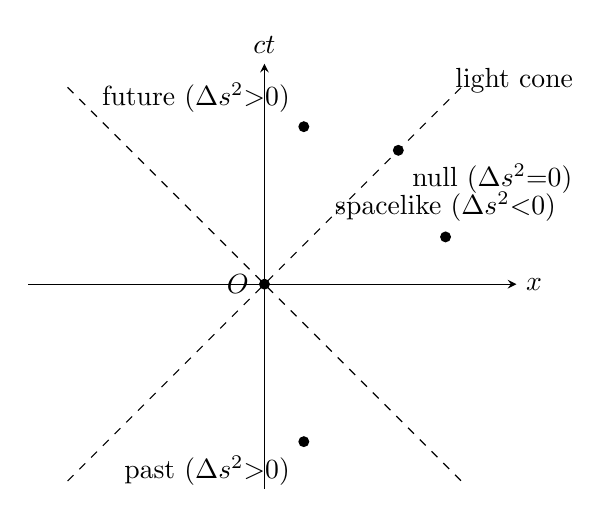
\begin{tikzpicture}[>=stealth, scale=1.0]
  \draw[->] (-3,0) -- (3.2,0) node[right] {$x$};
  \draw[->] (0,-2.6) -- (0,2.8) node[above] {$ct$};
  \draw[dashed] (-2.5,-2.5) -- (2.5,2.5);
  \draw[dashed] (-2.5,2.5) -- (2.5,-2.5);
  \node[above right] at (2.3,2.3) {light cone};
  \node[circle,fill,inner sep=1.4pt,label={above left:{future ($\Delta s^2{>}0$)}}] at (0.5,2.0) {};
  \node[circle,fill,inner sep=1.4pt,label={below left:{past ($\Delta s^2{>}0$)}}] at (0.5,-2.0) {};
  \node[circle,fill,inner sep=1.4pt,label={above:{spacelike ($\Delta s^2{<}0$)}}] at (2.3,0.6) {};
  \node[circle,fill,inner sep=1.4pt,label={below right:{null ($\Delta s^2{=}0$)}}] at (1.7,1.7) {};
  \node[circle,fill,inner sep=1.4pt,label={left:{$O$}}] at (0,0) {};
\end{tikzpicture}
\end{center}

\noindent\textbf{When is $Y^\mu X_\mu=0$?} Three independent cases:
\begin{enumerate}
\item One of the 4-vectors vanishes: $Y^\mu=0$ or $X^\mu=0$.
\item Both are null and parallel: $Y^\mu Y_\mu = X^\mu X_\mu = 0$ with $Y^\mu \propto X^\mu$.
\item One is timelike (or null) and the other spacelike (or null), oriented so the spatial overlap cancels the temporal product --- i.e.\ a genuinely orthogonal Minkowski pair.
\end{enumerate}
A timelike 4-vector cannot be orthogonal to another timelike 4-vector (their inner product retains the sign of $c^2\Delta t^2$).

\noindent\textbf{Pairs among $A,K,J$.}

4-acceleration vs.\ 4-velocity satisfies $A^\mu U_\mu=0$ identically (differentiate $U^\mu U_\mu=c^2$).

For a charged particle of rest charge density $\rho_0$, $J^\mu = \rho_0 U^\mu \propto U^\mu$. Hence
\[ A^\mu J_\mu = \rho_0\, A^\mu U_\mu = 0. \]
\[ \boxed{\;A\cdot J = 0\ \text{always}.\;} \]

\noindent For $K$ (photon, null) versus $A$ (spacelike): generically $A^\mu K_\mu\neq 0$ unless special alignment. Likewise $K\cdot J\neq 0$ in general (a charge moving relative to the photon will see a nonzero phase rate). So only $A\cdot J=0$ is guaranteed.

\subsection*{(b) 4-momentum, 4-acceleration, parallel case}

\textbf{Problem.} Define $\bm P$, $\bm A$. Compute $P^\mu P_\mu$. Show $A^\mu A_\mu=\gamma^6 a^2$ when $\bm v\parallel\bm a$.

Definitions:
\[ P^\mu = m U^\mu = (\gamma mc,\gamma m\bm v),\qquad A^\mu = \dv{U^\mu}{\tau} = \gamma\dv{U^\mu}{t}. \]
Compute $P^\mu P_\mu$:
\[ P^\mu P_\mu = \gamma^2 m^2 c^2 - \gamma^2 m^2 v^2. \]
Factor $\gamma^2 m^2$:
\[ P^\mu P_\mu = \gamma^2 m^2 (c^2-v^2). \]
Use $\gamma^2(c^2-v^2)=c^2$:
\[ \boxed{\;P^\mu P_\mu = m^2 c^2.\;} \]

\noindent\textbf{4-acceleration with $\bm v\parallel\bm a$.} Spatial 4-velocity $\bm u=\gamma\bm v$. Then
\[ \dv{u^0}{t} = c\,\dot\gamma,\qquad \dv{\bm u}{t} = \dot\gamma\bm v + \gamma\bm a. \]
Compute $\dot\gamma$ for $\bm v\parallel\bm a$:
\[ \dot\gamma = \dv{t}\!\bigl[(1-v^2/c^2)^{-1/2}\bigr] = \gamma^3 \frac{\bm v\!\cdot\!\bm a}{c^2} = \gamma^3 \frac{va}{c^2}. \]
Then
\[ A^0 = \gamma\dot\gamma c = \gamma^4\frac{va}{c}, \qquad \bm A = \gamma\bigl(\dot\gamma\bm v + \gamma\bm a\bigr) = \gamma^4\frac{v^2 a}{c^2}\hat{\bm a} + \gamma^2 a\hat{\bm a}. \]
Simplify $|\bm A|$:
\[ |\bm A| = \gamma^2 a\Bigl(\gamma^2\frac{v^2}{c^2}+1\Bigr) = \gamma^2 a\cdot\gamma^2 = \gamma^4 a. \]
Used $1+\gamma^2 v^2/c^2 = \gamma^2$. Compute the invariant:
\[ A^\mu A_\mu = (A^0)^2 - |\bm A|^2 = \gamma^8\frac{v^2 a^2}{c^2} - \gamma^8 a^2. \]
Factor:
\[ A^\mu A_\mu = \gamma^8 a^2\Bigl(\frac{v^2}{c^2}-1\Bigr) = -\gamma^8 a^2/\gamma^2. \]
\[ \boxed{\;A^\mu A_\mu = -\gamma^6 a^2.\;} \]
The magnitude $|A^\mu A_\mu|=\gamma^6 a^2$ as required (sign reflects $A$ being spacelike).

\subsection*{(c) Inverse-square central force: energy conservation}

\textbf{Problem.} For $\bm f = \alpha\bm r/r^3$, derive $\gamma mc^2 - \alpha/r = \text{const}$.

Relativistic 2nd law (rest mass preserved):
\[ \dv{t}(\gamma m\bm v) = \bm f. \]
Energy equation:
\[ \dv{t}(\gamma mc^2) = \bm f\!\cdot\!\bm v. \]
Insert force:
\[ \bm f\!\cdot\!\bm v = \frac{\alpha}{r^3}\bm r\!\cdot\!\bm v. \]
Identify $\bm r\!\cdot\!\bm v = r\dot r$:
\[ \bm f\!\cdot\!\bm v = \frac{\alpha\dot r}{r^2}. \]
Rewrite as total derivative:
\[ \frac{\alpha\dot r}{r^2} = -\dv{t}\!\Bigl(\frac{\alpha}{r}\Bigr). \]
Combine:
\[ \dv{t}\!\Bigl(\gamma mc^2 + \frac{\alpha}{r}\Bigr) = 0. \]
Hence (for attractive force $\alpha<0$, or the sign convention with potential $-\alpha/r$):
\[ \boxed{\;\gamma mc^2 - \frac{\alpha}{r} = \text{const}.\;} \]
\textit{Example.} Coulomb attraction between an electron and a proton: $\alpha = -e^2/(4\pi\epsilon_0)$ (or gravitational $\alpha=-GMm$ in the weak-field Newtonian limit).

\subsection*{(d) Electron accelerated across a 5 m gap, $E=\SI{10}{MV/m}$}

\textbf{Problem.} Find $\gamma$ at exit, time of flight, sketch $\gamma(t),\beta(t)$, $\Delta\beta$ if field reduced 20\%, and proton case.

Energy gain (work-energy theorem):
\[ \gamma mc^2 = mc^2 + eEL. \]
Solve for $\gamma$:
\[ \gamma = 1 + \frac{eEL}{mc^2}. \]
Insert numbers ($mc^2=\SI{0.511}{MeV}$, $eEL = \SI{10}{MeV/m}\times\SI{5}{m}=\SI{50}{MeV}$):
\[ \gamma = 1 + \frac{50}{0.511} = 1 + 97.85. \]
\[ \boxed{\;\gamma\approx 98.85\;} \]

\noindent\textbf{Time of flight.} Equation of motion (constant force, 1-D):
\[ \dv{t}(\gamma m v) = eE. \]
Integrate from rest:
\[ \gamma m v = eEt. \]
Square and use $\gamma^2 v^2 = c^2(\gamma^2-1)$:
\[ m^2 c^2(\gamma^2-1) = (eEt)^2. \]
Solve for $\gamma(t)$:
\[ \gamma(t) = \sqrt{1+\Bigl(\frac{eEt}{mc}\Bigr)^2}. \]
Position from $\dv*{x}{t}=v=c\sqrt{1-1/\gamma^2}$:
\[ x(t) = \frac{mc^2}{eE}\Bigl[\sqrt{1+(eEt/mc)^2}-1\Bigr]. \]
Set $x=L$ and solve:
\[ \sqrt{1+(eEt/mc)^2} = 1 + \frac{eEL}{mc^2} = \gamma. \]
Square:
\[ \Bigl(\frac{eEt}{mc}\Bigr)^2 = \gamma^2-1. \]
Solve $t$:
\[ t = \frac{mc}{eE}\sqrt{\gamma^2-1}. \]
Numerical: $\sqrt{\gamma^2-1}=\sqrt{98.85^2-1}\approx 98.84$, $mc^2/(eE)=\SI{0.511}{MeV}/\SI{10}{MV/m}=\SI{0.0511}{m}$, so $mc/(eE)=\SI{0.0511}{m}/c$:
\[ t = \frac{\SI{0.0511}{m}}{c}\times 98.84 = \frac{\SI{5.05}{m}}{c}. \]
\[ \boxed{\;t \approx \SI{1.69e-8}{s}\approx \SI{16.9}{ns}.\;} \]

\begin{center}
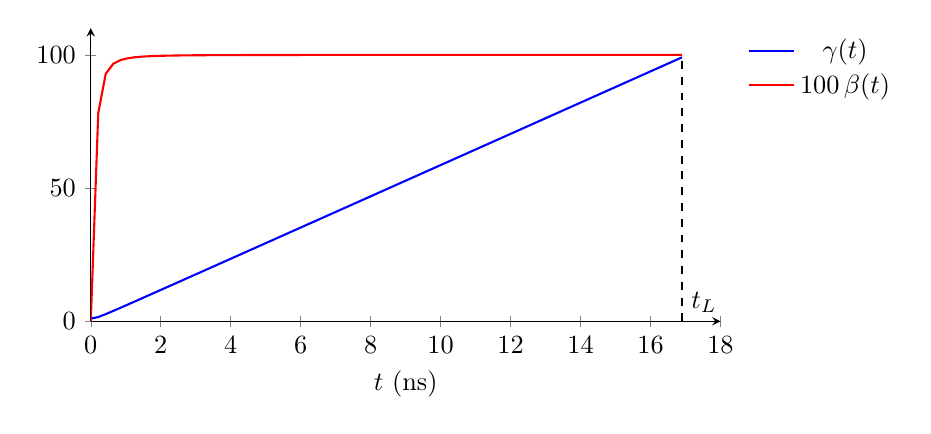
\begin{tikzpicture}[>=stealth, scale=0.95]
  \begin{axis}[
    width=10cm,height=5.5cm,
    xlabel={$t$ (ns)}, ylabel={},
    xmin=0, xmax=18, ymin=0, ymax=110,
    axis lines=left,
    legend pos=outer north east,
    legend style={draw=none}
  ]
    \addplot[domain=0:16.9, samples=80, thick, blue]
      ({x},{sqrt(1+(0.5*x/0.0852)^2)*0+sqrt(1+(x/0.1706)^2)});
    \addlegendentry{$\gamma(t)$}
    \addplot[domain=0:16.9, samples=80, thick, red]
      ({x},{100*sqrt(1-1/(1+(x/0.1706)^2))});
    \addlegendentry{$100\,\beta(t)$}
    \draw[dashed] (axis cs:16.9,0)--(axis cs:16.9,98.85);
    \node[anchor=south west] at (axis cs:16.9,0) {$t_L$};
  \end{axis}
\end{tikzpicture}
\end{center}

\noindent\textbf{Field reduced by 20\% ($E\to 0.8E$).} New $\gamma' = 1+0.8\times 97.85 = 79.28$. Both $\beta$ and $\beta'$ are very close to $1$:
\[ 1-\beta = \frac{1}{2\gamma^2} = \frac{1}{2\times 98.85^2} = \SI{5.12e-5}{},\quad 1-\beta' = \frac{1}{2\times 79.28^2} = \SI{7.96e-5}{}. \]
\[ \boxed{\;\Delta\beta \approx -\SI{2.8e-5}{} \;\text{(decrease)}.\;} \]

\noindent\textbf{Proton instead.} $m_p c^2 = \SI{938.3}{MeV}\gg \SI{50}{MeV}$, so non-relativistic:
\[ \gamma_p = 1 + \frac{50}{938.3} = 1.053. \]
\[ \beta_p = \sqrt{1-1/\gamma_p^2} = 0.314. \]
\[ \boxed{\;\gamma_p\approx 1.05,\ \beta_p\approx 0.31.\;} \]

% =====================================================================
\section*{Question 2 --- Photons, decays, fields, mirror reflection}

\subsection*{(a) Photon 4-wavevector, phase invariance}

\textbf{Problem.} Components of $\bm K$, dispersion, $v_\text{ph}$ and $v_g$, show $\phi$ is Lorentz-invariant; is $v_\text{ph}$ invariant?

4-wavevector:
\[ K^\mu = (\omega/c,\bm k),\qquad \omega = c|\bm k|. \]
Null condition (vacuum):
\[ K^\mu K_\mu = \omega^2/c^2 - |\bm k|^2 = 0. \]
Phase velocity (along $\hat{\bm k}$):
\[ v_\text{ph} = \omega/|\bm k| = c. \]
Group velocity:
\[ \bm v_g = \nabla_{\bm k}\omega = c\hat{\bm k},\qquad |\bm v_g|=c. \]
Phase of plane wave:
\[ \phi(\bm r,t) = \bm k\!\cdot\!\bm r - \omega t = -K^\mu X_\mu. \]
A contraction of two 4-vectors is a Lorentz scalar:
\[ \boxed{\;\phi = -K^\mu X_\mu \text{ is Lorentz-invariant.}\;} \]

\noindent\textbf{Is $v_\text{ph}$ Lorentz-invariant?} For a vacuum photon, $\omega'/|\bm k'|=c$ in every frame, so yes --- but only because $c$ is the universal speed limit. In a medium with $v_\text{ph}\neq c$, a Lorentz boost generally changes both $\omega$ and $|\bm k|$ such that $v_\text{ph}$ is \emph{not} invariant. So:
\[ \boxed{\;v_\text{ph}=c\text{ in vacuum: invariant. In a medium: not invariant.}\;} \]

\subsection*{(b) Forbidden and allowed photon processes}

\textbf{Problem.} Can $\gamma\to m+\gamma'$? Photon-photon $\to e^+e^-$: minimum number, threshold energy.

\textbf{Decay $\gamma\to m+\gamma'$.} 4-momentum conservation:
\[ K_1^\mu = P_m^\mu + K_2^\mu. \]
Square (use $K_1^\mu K_{1\mu}=K_2^\mu K_{2\mu}=0$, $P_m^\mu P_{m\mu}=m^2c^2$):
\[ 0 = m^2 c^2 + 2 P_m^\mu K_{2\mu}. \]
Solve:
\[ P_m^\mu K_{2\mu} = -\tfrac{1}{2}m^2 c^2. \]
In rest frame of $m$: $P_m=(mc,\bm 0)$, $K_2=(\omega_2/c,\bm k_2)$, so $P\!\cdot\!K_2 = m\omega_2 \geq 0$, contradicting the negative requirement (with metric $(+,-,-,-)$ and a real positive $\omega_2$). Equivalently, work in the $m$ rest frame: 3-momentum requires $\bm k_1=\bm k_2$, but then $\omega_1=\omega_2$ and energy conservation gives $mc^2=0$.
\[ \boxed{\;\text{Forbidden: a single photon cannot decay into }m+\gamma.\;} \]

\noindent\textbf{Photon-photon $\to e^+e^-$.} A single photon has $K^\mu K_\mu=0$ and cannot create a massive system ($P^2=(2m_e c)^2>0$) by itself. Two photons suffice if they are not collinear:
\[ (K_1+K_2)^\mu (K_1+K_2)_\mu = 2 K_1^\mu K_{2\mu} \geq (2m_e c)^2. \]
\[ \boxed{\;\text{Minimum: }2\text{ photons.}\;} \]

\noindent\textbf{Threshold.} Equal frequencies, head-on $\bm k_1=-\bm k_2$, $|\bm k_1|=|\bm k_2|=\omega/c$:
\[ K_1^\mu K_{2\mu} = \omega^2/c^2 - \bm k_1\!\cdot\!\bm k_2 = \omega^2/c^2 + \omega^2/c^2 = 2\omega^2/c^2. \]
Threshold ($e^+e^-$ produced at rest in CM):
\[ 2\cdot 2\omega^2/c^2 = (2m_e c)^2. \]
Solve:
\[ \omega = m_e c^2/\hbar. \]
Photon energy:
\[ E_\gamma = \hbar\omega = m_e c^2 = \SI{0.511}{MeV}. \]
\[ \boxed{\;E_\gamma^\text{min} = m_e c^2 \approx \SI{0.511}{MeV}\text{ per photon.}\;} \]

\subsection*{(c) Conserved 4-momentum components in $\bm E$ or $\bm B$ field}

\textbf{Problem.} Electron with $\bm v_0=(v_0,0,0)$. Which $P^\mu$ are conserved for (i) $\bm E=(E_x,0,0)$, (ii) $\bm B=(0,B_y,0)$.

Lorentz force:
\[ \dv{\bm p}{t} = e(\bm E + \bm v\times\bm B),\qquad \dv{E}{t} = e\bm E\!\cdot\!\bm v. \]

\textbf{(i) $\bm E=(E_x,0,0)$, no $\bm B$.} The force is $eE_x\hat{\bm x}$:
\[ \dv{p_y}{t}=0,\qquad \dv{p_z}{t}=0. \]
Energy is \emph{not} conserved ($\bm E\!\cdot\!\bm v = E_x v_x \neq 0$). So
\[ \boxed{\;P^y,\, P^z\text{ conserved}; P^0,\,P^x\text{ not.}\;} \]
Initial conditions give $p_y=p_z=0$ throughout.

\textbf{(ii) $\bm B=(0,B_y,0)$, no $\bm E$.} Magnetic force does no work:
\[ \dv{E}{t}=0\ \Rightarrow\ P^0\text{ conserved.} \]
$\bm v\times\bm B$ has no $y$-component when $\bm v$ has no $y$-component (initially $\bm v=(v_0,0,0)$). Check that $v_y$ remains zero: starting $\bm v=(v_x,0,v_z)$ stays in the $xz$-plane:
\[ \bm v\times\bm B = (v_x,0,v_z)\times(0,B_y,0) = (-v_z B_y,0,v_x B_y). \]
No $y$-component generated, so $p_y$ stays zero --- conserved.
\[ \boxed{\;P^0\text{ and }P^y\text{ conserved}; P^x,P^z\text{ rotate (circular motion).}\;} \]

\subsection*{(d) Reflection from a relativistic mirror}

\textbf{Problem.} Mirror moves at $\beta_x=0.99$ along $\hat{\bm x}$. Lab photon $\lambda_1=\SI{1}{\mu m}$. In mirror frame $\bm k'=(-k'_x,k'_y,0)$ with $|k'_x|=|k'_y|$. Find lab reflection angle and reflected $\lambda_2$.

\noindent\textbf{Step 1: Lorentz factor.} $\gamma = 1/\sqrt{1-0.99^2}=7.0888$.

\noindent\textbf{Step 2: Lab incident $\bm K_1$.} In mirror frame, $|k'_x|=|k'_y|$ with $k'_x<0$; the photon moves in $-\hat{\bm x}$ direction (against mirror velocity), as stated:
\[ K_1'^\mu = (\omega'/c)\,(1,-1/\sqrt{2},1/\sqrt{2},0),\qquad \omega' = c\sqrt{k'^2_x+k'^2_y}=c|k'_x|\sqrt{2}. \]
Boost to lab (frame $S$ moves with mirror velocity $+v\hat{\bm x}$ relative to $S$, so $S'$ at velocity $+v$ relative to $S$; the inverse boost from $S'\to S$ uses $-v$, i.e.\ $K^\mu = \Lambda^\mu_{\ \nu}(+v) K'^\nu$):
\[ \omega_1/c = \gamma(\omega'/c + \beta\, k'_x) = \gamma(\omega'/c)(1-\beta/\sqrt{2}). \]
\[ k_{1x} = \gamma(k'_x + \beta\omega'/c) = \gamma(\omega'/c)(\beta - 1/\sqrt{2}). \]
\[ k_{1y} = k'_y = (\omega'/c)/\sqrt{2}. \]
Numerical with $\beta=0.99$, $\gamma=7.0888$, $1/\sqrt 2=0.7071$:
\[ \omega_1/c = 7.0888\,(\omega'/c)(1-0.7000) = 2.127\,\omega'/c. \]
But we want to use the given $\lambda_1=\SI{1}{\mu m}$, so this fixes $\omega'$:
\[ \omega' = \omega_1/2.127. \]

\noindent\textbf{Step 3: Reflection in mirror frame.} A perfect mirror flips the normal component of $\bm k'$:
\[ K_2'^\mu = (\omega'/c)\,(1,+1/\sqrt 2,1/\sqrt 2,0). \]
Reflection angle in mirror frame is $45^\circ$ from normal.

\noindent\textbf{Step 4: Boost reflected photon back to lab.}
\[ \omega_2/c = \gamma(\omega'/c + \beta k'_{2x}) = \gamma(\omega'/c)(1+\beta/\sqrt 2). \]
\[ k_{2x} = \gamma(k'_{2x} + \beta\omega'/c) = \gamma(\omega'/c)(1/\sqrt 2 + \beta). \]
\[ k_{2y} = k'_{2y} = (\omega'/c)/\sqrt 2. \]
Numerics:
\[ \omega_2/c = 7.0888\,(\omega'/c)(1+0.7071) = 12.107\,\omega'/c. \]
Frequency ratio:
\[ \omega_2/\omega_1 = 12.107/2.127 = 5.692. \]
Wavelength of reflected photon:
\[ \lambda_2 = \lambda_1\,\omega_1/\omega_2 = \SI{1}{\mu m}/5.692. \]
\[ \boxed{\;\lambda_2 \approx \SI{0.176}{\mu m} \approx \SI{176}{nm}.\;} \]

\noindent\textbf{Reflection angle in lab.} Measure from $+\hat{\bm x}$ (mirror normal direction):
\[ \tan\theta_2 = k_{2y}/k_{2x} = \frac{1/\sqrt 2}{\gamma(1/\sqrt 2+\beta)} = \frac{0.7071}{7.0888\times 1.6971}. \]
Compute denominator:
\[ 7.0888\times 1.6971 = 12.030. \]
So
\[ \tan\theta_2 = 0.7071/12.030 = 0.05878. \]
\[ \boxed{\;\theta_2 = \arctan(0.0588) \approx 3.36^\circ\;} \]
The reflected photon emerges almost along $+\hat{\bm x}$ (relativistic beaming towards mirror motion direction).

% =====================================================================
\section*{Question 3 --- Bounds, Compton, periodic-field undulator}

\subsection*{(a) Bounds on forces, $v_\text{ph}$; Compton shift}

\textbf{Problem.} Bounds on forces/accelerations? On phase velocity? Derive Compton shift.

\textbf{No upper bound on force or acceleration.} Special relativity bounds the \emph{velocity} of a massive particle ($v<c$), but $\bm a = \de\bm v/\de t$ can be arbitrarily large in transient regimes; only the integrated speed-gain is constrained. For force, $\bm f = \de\bm p/\de t$ is similarly unbounded.

\noindent\textbf{Phase velocity is unbounded.} $v_\text{ph}=\omega/|\bm k|$ in a medium can exceed $c$ (e.g.\ X-rays in matter, plasma above $\omega_p$). The bound is on the group velocity / signal propagation, not phase.

\noindent\textbf{Compton shift.} Initial: photon $K=(\omega/c)(1,\hat{\bm n})$, electron at rest $P_e=(m_e c,\bm 0)$. After: photon $K'=(\omega'/c)(1,\hat{\bm n}')$, electron $P_e'$. Conservation:
\[ K + P_e = K' + P_e'. \]
Rearrange and square:
\[ (P_e + K - K')^\mu (P_e+K-K')_\mu = P_e'^\mu P_{e\mu}'. \]
Use $P_e^2 = P_e'^2 = m_e^2 c^2$, $K^2=K'^2=0$:
\[ m_e^2 c^2 + 2 P_e\!\cdot\!K - 2 P_e\!\cdot\!K' - 2 K\!\cdot\!K' = m_e^2 c^2. \]
Cancel $m_e^2 c^2$:
\[ P_e\!\cdot\!(K-K') = K\!\cdot\!K'. \]
Evaluate (rest frame $P_e=(m_e c,\bm 0)$):
\[ P_e\!\cdot\!K = m_e\omega,\quad P_e\!\cdot\!K' = m_e\omega',\quad K\!\cdot\!K' = (\omega\omega'/c^2)(1-\cos\theta). \]
Substitute:
\[ m_e(\omega-\omega') = (\omega\omega'/c^2)(1-\cos\theta). \]
Divide by $m_e\omega\omega'$:
\[ \frac{1}{\omega'}-\frac{1}{\omega} = \frac{1-\cos\theta}{m_e c^2}. \]
Convert to wavelength $\lambda = 2\pi c/\omega$:
\[ \boxed{\;\lambda' - \lambda = \frac{2\pi\hbar}{m_e c}(1-\cos\theta) = \lambda_C(1-\cos\theta)\;} \]
with Compton wavelength $\lambda_C = h/m_e c \approx \SI{2.43}{pm}$.

\subsection*{(b) Distance between two photons in $S'$}

\textbf{Problem.} Two photons separated by $x_0$ along $\hat{\bm x}$ in $S$. Find separation in $S'$ moving with $\bm v=(v_x,0,0)$.

The two photons are at events $E_1=(ct_0,x_0,0,0)$ and $E_2=(ct_0,0,0,0)$ at lab time $t_0$. In $S'$ these events do not occur simultaneously; the photons are points propagating along null worldlines, so we need the spatial separation between them in $S'$ measured at a single $S'$-time.

A photon has worldline $x = x_a + ct$ (forward-moving); both photons have parallel null worldlines $x_1 = x_0+ct$, $x_2 = ct$. The separation $x_1 - x_2 = x_0$ is constant in $S$. Apply Lorentz transformation: at fixed $t'$, find $\Delta x'$.

For each photon $K^\mu = (\omega_a/c)(1,1,0,0)$, the photon worldline parametrically transforms; in $S'$ (boost $+v$):
\[ x'_a = \gamma(x_a - vt),\qquad t'_a = \gamma(t - v x_a/c^2). \]
Solve $t_a$ at fixed $t'$: $t = (t' + v x_a/c^2)/\gamma$. Substitute:
\[ x'_a = \gamma\bigl(x_a - v(t'+vx_a/c^2)/\gamma\bigr) = \gamma x_a(1-v^2/c^2) - vt' = x_a/\gamma - vt'. \]
Difference:
\[ \Delta x' = (x_{1,a}-x_{2,a})/\gamma\Bigr|_{\text{at fixed }t}. \]
But this measures separation along the photons' shared null trajectory at constant lab time. The cleaner way: the photons' worldline parameter $x_a$ (lab-frame $x$-intercept) is Lorentz-mapped via the Doppler factor for null separations.

Use the invariant interval. $\Delta X^\mu = (0,x_0,0,0)$ between simultaneous $S$-events:
\[ \Delta X'^0 = -\gamma\beta x_0,\qquad \Delta X'^1 = \gamma x_0. \]
The events are not simultaneous in $S'$ ($\Delta t' = -\gamma\beta x_0/c \neq 0$). To get the $S'$-spatial separation between the photons at a single $S'$-time, slide one photon along its null worldline by $\Delta t'$:
\[ \Delta x'_\text{measured} = \gamma x_0 - c\,\Delta t' = \gamma x_0 - c(-\gamma\beta x_0/c) = \gamma x_0(1+\beta). \]
\[ \boxed{\;\Delta x' = x_0\,\gamma(1+\beta) = x_0\sqrt{\frac{1+\beta}{1-\beta}}.\;} \]
This is the relativistic Doppler factor for a separation along the propagation direction --- consistent with photons being "stretched apart" when the observer recedes.

\subsection*{(c) Head-on Compton: $\lambda_2 \approx \lambda_1/(4\gamma^2)$}

\textbf{Problem.} Electron and photon counter-propagate; head-on backscatter. Show $\lambda_2 \approx \lambda_1/(4\gamma^2)$ when $\hbar\omega\ll m_e c^2$. Numerical for $\beta=0.999$, $\lambda_1=\SI{8}{\mu m}$.

\textbf{Method: Doppler shift twice.} In electron rest frame the Compton shift on a low-energy photon is negligible (because $\hbar\omega'\ll m_e c^2$): $\omega'_\text{out}\approx \omega'_\text{in}$.

Doppler shift lab $\to$ electron rest frame (head-on collision, photon moves $-\hat{\bm x}$, electron at $+\hat{\bm x}$ velocity):
\[ \omega' = \gamma(1+\beta)\omega_1. \]
In rest frame, backscatter: outgoing photon at $+\hat{\bm x}$. Doppler back to lab:
\[ \omega_2 = \gamma(1+\beta)\omega'. \]
Combine:
\[ \omega_2 = \gamma^2(1+\beta)^2\,\omega_1. \]
Ultra-relativistic: $1+\beta \to 2$, $1-\beta\approx 1/(2\gamma^2)$:
\[ \omega_2 \approx 4\gamma^2\omega_1. \]
Wavelength:
\[ \boxed{\;\lambda_2 \approx \lambda_1/(4\gamma^2).\;} \]

\noindent\textbf{Numerical.} $\beta=0.999$:
\[ \gamma = 1/\sqrt{1-0.999^2} = 1/\sqrt{0.001999} = 22.366. \]
\[ 4\gamma^2 = 4\times 500.2 = 2000.8. \]
\[ \lambda_2 = \SI{8}{\mu m}/2000.8. \]
\[ \boxed{\;\lambda_2 \approx \SI{4.0}{nm}.\;} \]

\subsection*{(d) Plane EM wave: $A^\mu$, $\bm E$, $\bm B$}

\textbf{Problem.} Plane wave $\omega$, $\bm k=(k_x,0,0)$. Write a possible $A^\mu$, find $\bm E,\bm B$.

Lorenz-gauge null 4-potential, transverse polarization along $\hat{\bm y}$:
\[ A^\mu = (0, 0, A_0\cos(k_x x - \omega t), 0). \]
Fields:
\[ \bm E = -\nabla\phi - \partial_t\bm A = -\partial_t\bm A\hat{\bm y} = -A_0\omega\sin(k_x x-\omega t)\hat{\bm y}. \]
Use $\omega=ck_x$:
\[ \bm E = -A_0 c k_x \sin(k_x x-\omega t)\hat{\bm y}. \]
\[ \bm B = \nabla\times\bm A. \]
Only $A_y$ depends on $x$:
\[ \bm B = (\partial_x A_y)\hat{\bm z} = -A_0 k_x \sin(k_x x-\omega t)\hat{\bm z}. \]
\[ \boxed{\;\bm E = -A_0 c k_x \sin(k_x x-\omega t)\hat{\bm y},\quad \bm B = -A_0 k_x \sin(k_x x-\omega t)\hat{\bm z}\;} \]
$|\bm E|=c|\bm B|$, and $\bm E\times\bm B$ along $+\hat{\bm x}$ as required.

\subsection*{(e) Periodic-field undulator: lab vs.\ electron rest frame}

\textbf{Problem.} Undulator $A^\mu = (\phi/c,\bm 0)$, $\phi=\phi_0\cos(k_u z)$. Electron with $\bm v=(0,0,v_z)$, ultra-relativistic. Find $\bm E,\bm B$ in lab and rest frame; is the field in the rest frame an EM wave?

\textbf{Lab frame.}
\[ \bm E = -\nabla\phi = \phi_0 k_u\sin(k_u z)\hat{\bm z},\qquad \bm B = \nabla\times\bm A = 0. \]
\[ \boxed{\;\bm E_\text{lab} = \phi_0 k_u\sin(k_u z)\hat{\bm z},\quad \bm B_\text{lab}=\bm 0.\;} \]
A purely electrostatic, longitudinal, $z$-periodic field.

\textbf{Electron rest frame ($z' = \gamma(z-v t)$, $t'=\gamma(t-vz/c^2)$).} Boost the field strength tensor. Boost direction parallel to $\bm E$, so the longitudinal $E_z$ is unchanged and a transverse $\bm B$ does not appear:
\[ E'_z = E_z,\qquad B'_\perp = -\gamma\beta\,(E\times \hat{\bm v})_\perp / c = 0. \]
So $\bm B'=0$ (boost along $\bm E$), but the spatial argument transforms:
\[ k_u z = k_u(\gamma z' + \gamma v t') = \gamma k_u z' + \gamma k_u v t'. \]
Define $k'_u = \gamma k_u$, $\omega' = \gamma k_u v \approx \gamma k_u c$ (ultra-relativistic):
\[ \bm E'(\bm r',t') = \phi_0 k_u\sin(k'_u z' + \omega' t')\hat{\bm z}'. \]
\[ \boxed{\;\bm E' = \phi_0 k_u \sin(\gamma k_u z' + \gamma k_u v\,t')\hat{\bm z}',\quad \bm B'=\bm 0.\;} \]

\noindent\textbf{Is this an EM wave?} A vacuum plane EM wave satisfies $|\bm E|=c|\bm B|$ with $\bm E\perp\bm k$, $\bm B\perp\bm k$, $\bm B\neq 0$. Here $\bm B'=0$ and $\bm E'\parallel\hat{\bm z}'$ (longitudinal to the propagation direction $\hat{\bm z}'$).
\[ \boxed{\;\text{Not an EM wave: longitudinal }\bm E,\ \bm B'=0.\;} \]
It is a longitudinal oscillating electric field --- the rest-frame view of a static periodic potential as seen by a co-moving observer (no radiation; it is not transverse).

% =====================================================================
\section*{Question 4 --- Polar/axial vectors, $F^{\mu\nu}$, capacitor}

\subsection*{(a) Polar vs.\ axial; $\bm E,\bm B$}

\textbf{Problem.} Define polar/axial 3-vectors. Are $\bm E,\bm B$ polar or axial? Justify via Lorentz force.

\textbf{Polar vector:} flips sign under spatial inversion $\bm r\to-\bm r$ (e.g.\ $\bm r,\bm v,\bm p,\bm E$).

\textbf{Axial (pseudo-) vector:} unchanged under inversion (e.g.\ $\bm L=\bm r\times\bm p$, $\bm B$, angular velocity).

Lorentz force $\bm F = q(\bm E + \bm v\times\bm B)$. Under parity:
\[ \bm F\to -\bm F,\quad q\bm E\to -q\bm E\ \Rightarrow\ \bm E\text{ is polar}. \]
\[ \bm v\times\bm B \to (-\bm v)\times \bm B \to -\bm v\times\bm B\quad\text{requires}\quad \bm B\to +\bm B. \]
So
\[ \boxed{\;\bm E\text{ polar},\ \bm B\text{ axial}.\;} \]

\subsection*{(b) 4-current, continuity, Lorentz force on a charge density}

\textbf{Problem.} Define $J^\mu$, write continuity, derive $f_\mu = J^\nu F_{\nu\mu}$, identify $f_0$.

4-current:
\[ J^\mu = \rho_0 U^\mu = (\rho c, \bm j),\qquad \bm j = \rho\bm v. \]
Continuity:
\[ \boxed{\;\partial_\mu J^\mu = 0 \quad\Leftrightarrow\quad \partial_t\rho + \nabla\!\cdot\!\bm j = 0.\;} \]
Lorentz force per unit volume:
\[ \bm f = \rho\bm E + \bm j\times\bm B. \]
Power per unit volume (rate of work done on charges):
\[ f^0 c = \bm j\!\cdot\!\bm E. \]

\noindent\textbf{Derive $f_\mu = J^\nu F_{\nu\mu}$.} Field tensor:
\[ F_{\nu\mu} = \partial_\nu A_\mu - \partial_\mu A_\nu,\qquad F^{0i}=-E_i/c,\ F^{ij}=-\epsilon_{ijk}B_k. \]
Compute $J^\nu F_{\nu\mu}$ for $\mu=i$ (spatial):
\[ J^\nu F_{\nu i} = J^0 F_{0 i} + J^j F_{j i}. \]
Insert components ($F_{0i}=E_i/c$, $F_{ji}=\epsilon_{jik}B_k$, $J^0=\rho c$, $J^j=j_j$):
\[ J^\nu F_{\nu i} = \rho E_i + (\bm j\times\bm B)_i = f_i. \]
Done.

\noindent\textbf{$f^0$ component:}
\[ f^0 = J^j F^{0}_{\ j} = (\bm j\!\cdot\!\bm E)/c. \]
\[ \boxed{\;f^0 = \bm j\!\cdot\!\bm E /c = \text{rate of work done by the field per unit volume, divided by }c.\;} \]
Physically: power density delivered by the EM field to the charges (the time component of the 4-force density).

\subsection*{(c) $F^{\alpha\beta}$ from given $A^\mu$}

\textbf{Problem.} $A^\mu = (0,A_0\cos(K\!\cdot\!X), A_0\sin(K\!\cdot\!X),0)$, $K=(\omega/c,0,0,k_z)$. Compute $F^{\alpha\beta}=\partial^\alpha A^\beta-\partial^\beta A^\alpha$.

Phase: $\Phi \equiv K^\mu X_\mu = \omega t - k_z z$ (using metric $(+,-,-,-)$, $K\!\cdot\!X = (\omega/c)(ct) - k_z z$).

Components: $A^1=A_0\cos\Phi$, $A^2=A_0\sin\Phi$, $A^0=A^3=0$.

Derivatives ($\partial^0 = (1/c)\partial_t$, $\partial^i = -\partial_i$, $\partial_0\Phi = \omega/c$, $\partial_3\Phi = -k_z$):
\[ \partial^0 A^1 = (1/c)\partial_t A^1 = -A_0(\omega/c)\sin\Phi. \]
\[ \partial^0 A^2 = A_0(\omega/c)\cos\Phi. \]
\[ \partial^3 A^1 = -\partial_z A^1 = -A_0 k_z\sin\Phi. \]
\[ \partial^3 A^2 = A_0 k_z\cos\Phi. \]
\[ \partial^1 A^0 = \partial^2 A^0 = \partial^1 A^3 = \partial^2 A^3 = 0. \]
Antisymmetric tensor:
\[ F^{01} = \partial^0 A^1 - \partial^1 A^0 = -A_0(\omega/c)\sin\Phi. \]
\[ F^{02} = A_0(\omega/c)\cos\Phi. \]
\[ F^{31} = \partial^3 A^1 - \partial^1 A^3 = -A_0 k_z\sin\Phi. \]
\[ F^{32} = A_0 k_z\cos\Phi. \]
\[ F^{12} = \partial^1 A^2 - \partial^2 A^1 = 0. \]
Identify $\bm E$, $\bm B$ from $F^{0i}=-E_i/c$, $F^{ij}=-\epsilon_{ijk}B_k$:
\[ \bm E = (A_0\omega\sin\Phi,\, -A_0\omega\cos\Phi,\, 0). \]
\[ \bm B = (-A_0 k_z\cos\Phi,\, -A_0 k_z\sin\Phi,\, 0). \]
\[ \boxed{\;|\bm E|=A_0\omega,\ |\bm B|=A_0 k_z,\ |\bm E|=c|\bm B|,\ \bm E\!\cdot\!\bm B=0.\;} \]
Circularly polarised plane wave propagating along $+\hat{\bm z}$.

\subsection*{(d) Field transformation under boost}

\textbf{Problem.} $S'$ moves with 3-velocity $\bm v$ relative to $S$. Write $\bm E'$, $\bm B'$.

Decompose into components parallel ($\parallel$) and perpendicular ($\perp$) to $\bm v$:
\[ \bm E'_\parallel = \bm E_\parallel,\qquad \bm B'_\parallel = \bm B_\parallel. \]
\[ \boxed{\;\bm E'_\perp = \gamma(\bm E_\perp + \bm v\times\bm B)_\perp,\qquad \bm B'_\perp = \gamma\bigl(\bm B_\perp - (\bm v\times\bm E)/c^2\bigr)_\perp.\;} \]

\subsection*{(e) Capacitor + magnetic field}

\textbf{Problem.} Plates parallel to $yz$-plane, gap $d=\SI{0.1}{m}$, $E=\SI{100}{MV/m}$ between plates, electron launched from negative plate at rest. (i) Energy and velocity at the second plate; (ii) can a $\bm B$ prevent it hitting positive plate; (iii) direction; (iv) magnitude; (v) trajectory sketch.

\textbf{(i) Energy and velocity at the second plate.}

Energy gained:
\[ \Delta E = eEd = \SI{100}{MeV/m}\times \SI{0.1}{m} \times e \cdot 1 = \SI{10}{MeV}. \]
Wait: $E=\SI{100}{MV/m}\Rightarrow eE = \SI{100}{MeV/m}\cdot e/e = \SI{100}{MeV/m}$ (in eV-units). Times $d=\SI{0.1}{m}$:
\[ eEd = \SI{10}{MeV}. \]
Total energy:
\[ E_\text{tot} = m_e c^2 + 10 = 0.511 + 10 = \SI{10.511}{MeV}. \]
\[ \gamma = E_\text{tot}/m_e c^2 = 10.511/0.511 = 20.57. \]
\[ \beta = \sqrt{1-1/\gamma^2} = \sqrt{1-1/423.1} = \sqrt{0.99764} = 0.99882. \]
\[ \boxed{\;E_\text{kin}\approx \SI{10}{MeV},\ \gamma\approx 20.6,\ v\approx 0.999\,c.\;} \]

\textbf{(ii) Can $\bm B$ prevent it reaching the positive plate?}

Yes. A magnetic field perpendicular to the electron velocity bends its trajectory; if the field is strong enough, the gyroradius is smaller than the gap so that the electron curves back to the negative plate before hitting the positive plate.
\[ \boxed{\;\text{Yes --- a transverse }\bm B\text{ bends the electron back.}\;} \]

\textbf{(iii) Direction of $\bm B$.} Take electron initial $\bm v$ along $+\hat{\bm x}$. To bend it inside the $xz$ (or $xy$) plane back toward the negative plate, $\bm B$ must lie in the $yz$-plane (perpendicular to $\bm v$). Choosing $\bm B = B\hat{\bm y}$:
\[ \boxed{\;\bm B \parallel \hat{\bm y}\text{ (or }\hat{\bm z}\text{): perpendicular to }\bm v\text{ and to }\bm E.\;} \]
The electron then executes (modified) cyclotron motion in the $xz$-plane.

\textbf{(iv) Strength of $\bm B$ to stop the electron at $x=d$.}

Energy conservation in static fields ($\bm B$ does no work):
\[ \tfrac{1}{2}\text{(at any position }x): \gamma(x)m_e c^2 = m_e c^2 + eEx. \]
At the turn-back point the electron must have $v_x=0$. Use canonical momentum conservation: with $\bm B = B\hat{\bm y}$ and $\bm A = -Bx\hat{\bm z}$ (so $\bm B = \nabla\times\bm A = B\hat{\bm y}$), $A_z$ depends on $x$ only, and the system is independent of $z$:
\[ p_z + qA_z = \text{const},\qquad q=-e. \]
At launch: $p_z=0$, $x=0\Rightarrow A_z=0$:
\[ p_z(x) - e(-Bx) = 0\ \Rightarrow\ p_z(x) = -eBx. \]
Hmm sign: with $q=-e$ and $A_z = -Bx$, conservation of $p_z + q A_z$:
\[ p_z(x) + (-e)(-Bx) = 0\ \Rightarrow\ p_z(x) = -eBx. \]
At turn-around $v_x=0$, so $|p_z(x_\text{max})| = p_\text{tot}(x_\text{max}) = \gamma(x_\text{max})m_e v(x_\text{max})$.

Total momentum at $x$:
\[ p_\text{tot}(x) c = \sqrt{E_\text{tot}(x)^2 - (m_e c^2)^2},\quad E_\text{tot}(x) = m_e c^2 + eEx. \]
Set $|p_z| = p_\text{tot}$ at $x=x_\text{max}=d$:
\[ eBd = p_\text{tot}(d). \]
Solve:
\[ B = p_\text{tot}(d)/(ed). \]
At $x=d$: $E_\text{tot}=\SI{10.511}{MeV}$, so
\[ p_\text{tot} c = \sqrt{10.511^2 - 0.511^2} = \sqrt{110.48 - 0.261} = \sqrt{110.22} = \SI{10.499}{MeV}. \]
Hence $p_\text{tot} = \SI{10.499}{MeV}/c$. Convert:
\[ B = \frac{\SI{10.499}{MeV}/c}{e\cdot \SI{0.1}{m}} = \frac{10.499\times \SI{e6}{eV}}{c\,\SI{0.1}{m}\,e}\,\text{T-equivalent}. \]
Numerically using $1\,\text{T}\cdot c\cdot \SI{1}{m} = \SI{2.998e8}{V}$:
\[ B = \frac{p c}{e d c} = \frac{\SI{10.499e6}{V}}{\SI{2.998e8}{V/T\cdot m}\times \SI{0.1}{m}}. \]
Compute denominator:
\[ \SI{2.998e8}{}\times 0.1 = \SI{2.998e7}{V/T}. \]
\[ B = \SI{10.499e6}{}/\SI{2.998e7}{} = 0.3502\,\text{T}. \]
\[ \boxed{\;B \approx \SI{0.35}{T}.\;} \]

\textbf{(v) Trajectory sketch.}

The electron starts at the negative plate with $\bm v=\bm 0$. Initially $\bm B$ exerts no force; the $\bm E$-field accelerates it along $+\hat{\bm x}$. As $v_x$ grows, the magnetic force $-e\bm v\times\bm B = -e v_x\hat{\bm x}\times B\hat{\bm y} = -ev_xB\hat{\bm z}$ deflects it toward $-\hat{\bm z}$. The electron curves; if $B$ is exactly the threshold $\SI{0.35}{T}$ found above, $v_x\to 0$ at $x=d$ (just touching the positive plate momentarily), then it returns. Trajectory is a cycloidal arc concave toward $-\hat{\bm z}$.

\begin{center}
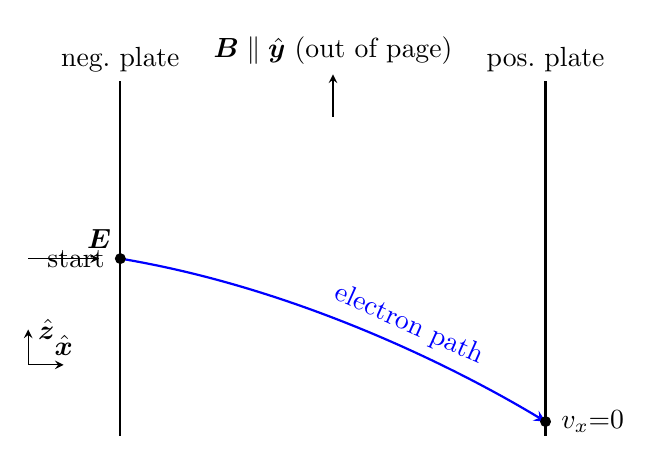
\begin{tikzpicture}[>=stealth, scale=0.9]
  \draw[thick] (0,-2.5) -- (0,2.5);
  \draw[thick] (6,-2.5) -- (6,2.5);
  \node[above] at (0,2.5) {neg.\ plate};
  \node[above] at (6,2.5) {pos.\ plate};
  \draw[->] (-1.3,0) -- (-0.3,0) node[above] {$\bm E$};
  \draw[->,thick,blue] (0,0) .. controls (3,-0.5) and (5.5,-2) .. (6,-2.3)
        node[pos=0.5, above, sloped] {electron path};
  \node[circle,fill,inner sep=1.4pt,label=left:{start}] at (0,0) {};
  \node[circle,fill,inner sep=1.4pt,label=right:{$v_x{=}0$}] at (6,-2.3) {};
  \draw[->] (3,2.0) -- (3,2.6) node[above] {$\bm B \parallel \hat{\bm y}$ (out of page)};
  \draw[->] (-1.3,-1.5) -- (-1.3,-1.0) node[right] {$\hat{\bm z}$};
  \draw[->] (-1.3,-1.5) -- (-0.8,-1.5) node[above] {$\hat{\bm x}$};
\end{tikzpicture}
\end{center}

If $B$ slightly exceeds threshold, the electron turns back before $x=d$ and executes a cycloidal drift along $-\hat{\bm z}$ between the plates (drift velocity $\bm v_d = \bm E\times\bm B/B^2$).

\end{document}
